\section{GPU benchmarks}
\begin{frame}[fragile]
  \frametitle{Hardware}
  \pause{}
  \begin{exampleblock}{\texttt{clinfo}}
\begin{verbatim}
Device Name                     NVIDIA GeForce GTX 1060
Max clock frequency             1733MHz
Preferred/native vector sizes
  char                                 1 / 1
  int                                  1 / 1
  float                                1 / 1
  double                               1 / 1
Global memory size              6373572608 (5.936GiB)
Local memory size               49152 (48KiB)
\end{verbatim}
  \end{exampleblock}
  \pause{}
  \begin{alertblock}{Does not support vector instructions}
    Only \alert{1} char/int/float/double OP per Processing Element
    (PE) per cycle
  \end{alertblock}
\end{frame}

\begin{frame}
  \frametitle{Performance estimation for
    \texttt{add\_char/add\_float}}
  \pause{}
  \begin{figure}[t]
    \centering 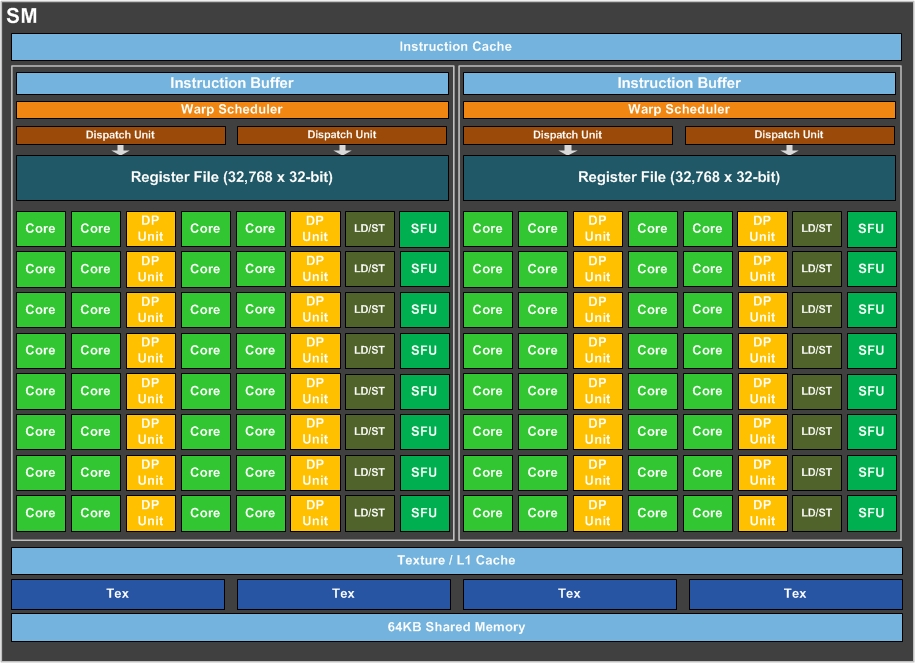
\includegraphics[height=5.5cm]{sm.png}
    % \caption{Architecture of an SM from Pascal Whitepaper}
  \end{figure}
  % \begin{block}{Assumptions}
  %   \begin{itemize}
  %   \item The GPU runs at max frequency (1.7GHz)
  %   \item Only our program runs on the GPU
  %   \end{itemize}
  % \end{block}
  \pause{}
  \begin{align*}
    \#OpPerSecond &= \#SM \times \#Cores \times Frequency      \\
                  &= 10 \times (64 + 32) \times 1.7 \\
                  &= \alert{1632~\mathit{G}}
  \end{align*}
\end{frame}

\begin{frame}[fragile]
  \frametitle{\texttt{add\_char} v1.0}
\begin{lstlisting}[basicstyle=\footnotesize]
kernel void
add_char (char scale)
{
  char sum = 1;
  sum += scale;
}

clEnqueueNDRangeKernel (cmd_queue, kernel, 1, 0,
                        &size, 0, 0, 0, 0);
\end{lstlisting}
  \pause{}p
  \begin{alertblock}{Results}
    For \lstinline{size = 1000 000 000}: \pause{}\alert{Only}
    \(67~\mathit{GOPS}\) \\
    \pause{} (Perhaps) software dimension is too big
  \end{alertblock}
\end{frame}

\begin{frame}[fragile]
  \frametitle{\texttt{add\_char} v2.0}
\begin{lstlisting}[basicstyle=\footnotesize]
kernel void
add_char (int iter, char scale)
{
  char sum = 1;
  for (int i = 0; i < iter; ++i)
      sum += scale;
}

int load_per_thd = 10000;
size_t dim = size / load_per_thd;
clSetKernelArg (kernel, 0, sizeof (int), &load_per_thd);
clEnqueueNDRangeKernel (cmd_queue, kernel, 1, 0,
                        &dim, 0, 0, 0, 0);
\end{lstlisting}
  \pause{}
  \begin{alertblock}{Results}
    For \lstinline{size = 1000 000 000}:
    \pause{}\(62500~\mathit{GOPS}\)!!! \\
    \pause{} However, changing \lstinline{iter} while having the same
    \lstinline{size} causes no change.
  \end{alertblock}
\end{frame}

\begin{frame}[fragile]
  \frametitle{\texttt{add\_char} v3.0}
  \pause{}
\begin{lstlisting}[basicstyle=\footnotesize]
kernel void
add_char (int iter, char scale, global char *out)
{
  char sum = 1;
  for (int i = 0; i < iter; ++i)
    {
      sum += scale;
    }
  out[get_global_id (0)] = sum;
}
\end{lstlisting}
  \begin{alertblock}{Results}
    For \lstinline{size = 1000 000 000}:
    \pause{}\(1390~\mathit{GOPS}\) \pause{}
    \begin{itemize}
    \item Close to the theoretical limit (\(1632~\mathit{GOPS}\))
    \end{itemize}
  \end{alertblock}
\end{frame}

\begin{frame}[fragile]
  \frametitle{\texttt{load\_seq}}
  \lstinputlisting[basicstyle=\footnotesize, linerange=41-50]{../gpubench/kernel.cl}
  \pause{}
  \begin{alertblock}{Results}
    Sequentially read an array of \(4~\mathit{GB}\)
    \begin{itemize}
    \item \(3.3~\mathit{GB/s}\)
    \item \(0.82~\mathit{GOPS}\)
    \end{itemize}
  \end{alertblock}
\end{frame}

\begin{frame}[fragile]
  \frametitle{\texttt{load\_rand}}
  \lstinputlisting[basicstyle=\footnotesize, linerange=52-61]{../gpubench/kernel.cl}
  \pause{}
  \begin{alertblock}{Results}
    Sequentially read an array of \(4~\mathit{GB}\)
    \begin{itemize}
    \item \(0.023~\mathit{GB/s}\)
    \item \(0.006~\mathit{GOPS}\)
    \end{itemize}
  \end{alertblock}
\end{frame}

\begin{frame}[fragile]
  \frametitle{\texttt{transfer\_data}}
\begin{lstlisting}[basicstyle=\footnotesize]
  char *array = malloc (sizeof (char) * size);
  cl_mem buf = CL_CHECK_R (
    clCreateBuffer (context, CL_MEM_READ_ONLY,
                    sizeof (char) * size, 0, &cl_err));
  CL_CHECK (clFinish (cmd_queue));
  START_TIMER (timer);
  CL_CHECK (
    clEnqueueWriteBuffer (cmd_queue, buf, 0, 0,
                          size, array, 0, 0, 0));
  CL_CHECK (clFinish (cmd_queue));
  END_TIMER (timer);
\end{lstlisting}
  \pause{}
  \begin{alertblock}{Results}
    Transfer an array of \(1~\mathit{GB}\) from CPU to GPU
    \begin{itemize}
    \item \(4.1~\mathit{GB/s}\)
    \end{itemize}
  \end{alertblock}
\end{frame}

%%% Local Variables:
%%% mode: latex
%%% TeX-master: "presentation"
%%% End:
